\documentclass[a4paper,12pt]{article}

\usepackage[T2A]{fontenc}			
\usepackage[utf8]{inputenc}			
\usepackage[english,russian]{babel}	

\usepackage[
bookmarks=true, colorlinks=true, unicode=true,
urlcolor=black,linkcolor=black, anchorcolor=black,
citecolor=black, menucolor=black, filecolor=black,
]{hyperref}

\usepackage{color}
\usepackage{caption}
\DeclareCaptionFont{white}{\color{black}}
\DeclareCaptionFormat{listing}{\colorbox{white}{\parbox{\textwidth}{#1#2#3}}}
\captionsetup[lstlisting]{format=listing,labelfont=white,textfont=white}

\usepackage{amsmath,amsfonts,amssymb,amsthm,mathtools} 
\usepackage{wasysym}

\usepackage{graphicx}
%\usepackage[cache=false]{minted}
\usepackage{cmap}
\usepackage{indentfirst}

\usepackage{listings} 
\usepackage{fancyvrb}

\usepackage{geometry}
\geometry{left=2cm}
\geometry{right=1.5cm}
\geometry{top=1cm}
\geometry{bottom=2cm}

\setlength{\parindent}{5ex}
\setlength{\parskip}{0.5em}

\usepackage{pgfplots}
\usetikzlibrary{datavisualization}
\usetikzlibrary{datavisualization.formats.functions}

\begin{document}
	\lstset{ %
		language=C,                 % выбор языка для подсветки (здесь это С)
		basicstyle=\small\sffamily, % размер и начертание шрифта для подсветки кода
		numbers=left,               % где поставить нумерацию строк (слева\справа)
		numberstyle=\tiny,           % размер шрифта для номеров строк
		stepnumber=1,                   % размер шага между двумя номерами строк
		numbersep=5pt,                % как далеко отстоят номера строк от подсвечиваемого кода
		backgroundcolor=\color{white}, % цвет фона подсветки - используем \usepackage{color}
		showspaces=false,            % показывать или нет пробелы специальными отступами
		showstringspaces=false,      % показывать или нет пробелы в строках
		showtabs=false,             % показывать или нет табуляцию в строках
		frame=single,              % рисовать рамку вокруг кода
		tabsize=2,                 % размер табуляции по умолчанию равен 2 пробелам
		captionpos=t,              % позиция заголовка вверху [t] или внизу [b] 
		breaklines=true,           % автоматически переносить строки (да\нет)
		breakatwhitespace=false, % переносить строки только если есть пробел
		escapeinside={\%*}{*)}   % если нужно добавить комментарии в коде
	}
	
	% Титульный лист
	\begin{figure}[h!]
		\begin{center}
			{
\includegraphics[scale = 0.4]{titul.jpg}}
			\label{titul}
		\end{center}
	\end{figure}
	
	\vspace*{15mm} 
	
	\huge
	\begin{center}
		Дисциплина: <<Функциональное и логическое программирование>>
	\end{center}
	\vspace*{15mm} 	
	
	\begin{center}
		Лабораторная работа №10
	\end{center}
	
	\vspace*{15mm} 	
	
	\large
	\begin{flushright}
		Студент: Левушкин И. К. \\
		Группа: ИУ7-62Б \\
		Преподаватели: Толпинская Н. Б., \\ Строганов Ю. В. \\
	\end{flushright}
	
	\vspace*{30mm}
	\begin{center}
		Москва, 2020 г.  
	\end{center}
	\thispagestyle{empty}
	
	
	\newpage
	
	\section*{6.7. Пусть list-of-list список, состоящий из списков. Написать функцию, которая вычисляет сумму длин всех элементов list-of-list, т.е. например для аргумента ((1 2) (3 4)) -> 4.  
	 }
 
 	\subsection*{Реализация задания}
 	
 	\begin{figure}[h!]
 		\begin{center}
 			{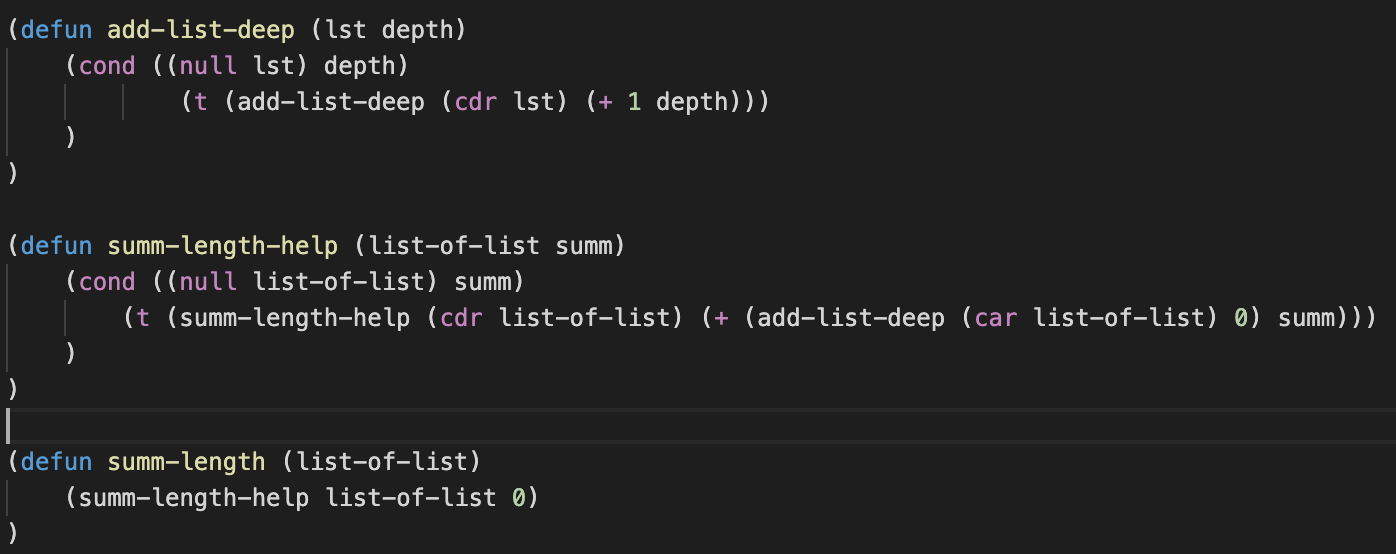
\includegraphics[scale = 0.7]{6.7.png}}
 			\label{ris:6.7}
 		\end{center}
 	\caption{Рекурсивная реализация функции, вычисляющей сумму длин всех элементов списка}
 	\end{figure}
 	
 	\subsection*{Назначение параметров функций}
 	
 	\begin{itemize}
 		\item Функция summ-length - функция-обретка, запускающая рекурсивную функцию summ-length-help с начальным параметром суммы summ = 0
 		\item Функция summ-length-help проверет, пустой ли список, если пустой, то возвращает summ, если нет, то подсчитывает длинну (глубину) очередного аргумента списка, вызывая при этом рекурсивную функцию add-list-deep с начальным параметром deep = 0
 		\item Функция add-list-deep считает глубину списка lst (до тех пор, пока lst не nil)
 	\end{itemize}
 	
 	\subsection*{Результаты работы}
 	
 	 	\begin{table} [h!]
 		\begin{center}
 			\begin{tabular}{|l|l|}
 				\hline
 				{\bf  Выражение} & {\bf Результат} \\
 				\hline
 				{'((1 2) (3 4))} & 4\\
 				\hline
 				{'((1 2) NIL (3 4))} & 4\\
 				\hline
 				{'((1 2) NIL (3 4 (5 6)))} & 5\\
 				\hline
 				{'()} & 0 \\
 				\hline
 				{'((3 4 5 6 7) () (1 2))} & 7\\
 				\hline
 			\end{tabular}  
 			\label{m2}
 		\end{center}
 	\end{table}
 	
 	 \newpage
 	
 	\section*{6.8. Написать рекурсивную версию (с именем reg-add) вычисления суммы чисел
заданного списка.
Например: (reg-add (2 4 6)) -> 12
 	}
 	
 	\subsection*{Реализация задания}
 	
 	 	Так как в условии задачи не сказано, является ли список-аргумент списком чисел, будем считать, что элементы списка - любые объекты.
 	
 	\begin{figure}[h!]
 		\begin{center}
 			{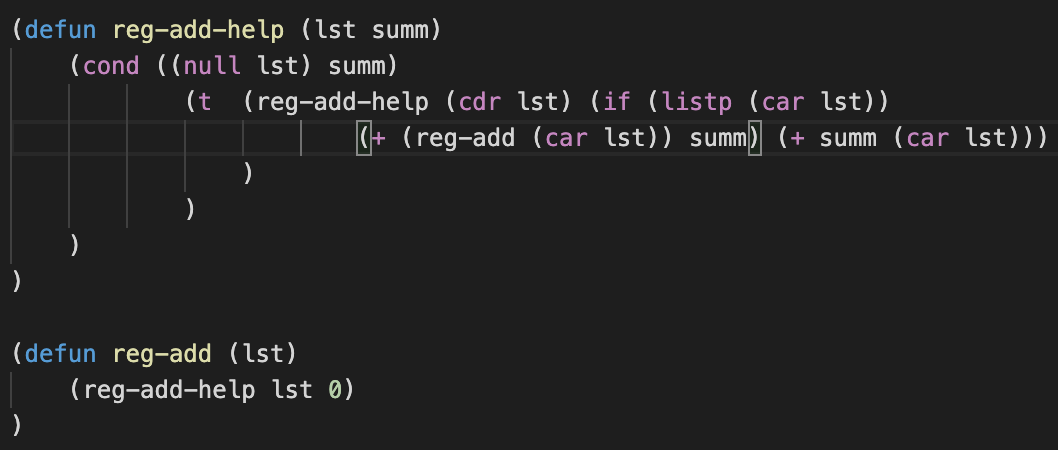
\includegraphics[scale = 1.0]{6.8.png}}
 			\label{ris:6.8}
 		\end{center}
 	\caption{Рекурсивная реализация функции reg-add}
 	\end{figure}
 	
 	\subsection*{Назначение параметров функций}
 	
 	\begin{itemize}
 		\item Функция reg-add - функция-обертка, запускающая рекурсивную функцию reg-add-help с начальным параметром summ = 0
 		\item Функция reg-add-help - функция, подсчитывающая сумму чисел заданного списка. Если очередной элемент списка является списком, считает сумму чисел уже внутреннего списка, запуская функцию reg-add для этого списка, и добавляет к уже имеющейся
 	\end{itemize}
 	
 	\subsection*{Результаты работы}
 	
 	 	 	\begin{table} [h!]
 		\begin{center}
 			\begin{tabular}{|l|l|}
 				\hline
 				{\bf  Выражение} & {\bf Результат} \\
 				\hline
 				{'(1 2 3 4 5 6)} & 21\\
 				\hline
 				{'(1 2 3 (5 6 7) 3 2)} & 29\\
 				\hline
 				{'(1 2 3 () 3 2)} & 11 \\
 				\hline
 				{'()} & 0\\
 				\hline
 			\end{tabular}  
 			\label{m2}
 		\end{center}
 	\end{table}
 	
 	\newpage
 	
 	\section*{6.9. Написать рекурсивную версию с именем recnth функции nth. 
 	}
 	
 	\subsection*{Реализация задания}
 	
 	\begin{figure}[h!]
 		\begin{center}
 			{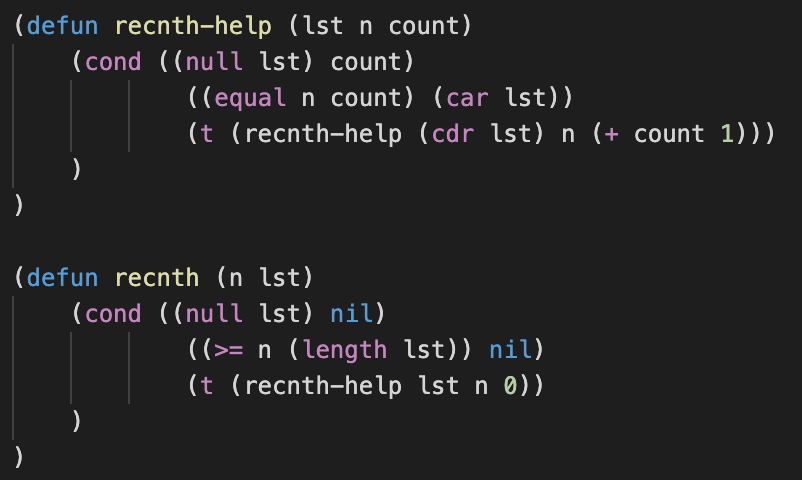
\includegraphics[scale = 1.0]{6.9.png}}
 			\label{ris:6.9}
 		\end{center}
 	\caption{Рекурсивная реализация функции recnth}
 	\end{figure}
 	
 	\subsection*{Назначение параметров функций}
 	
 	\begin{itemize}
 		\item Функция recnth - функция-обертка, проверяющая lst на пустой список и, меньше ли входной параметр n длины списка lst. Если не пуст и меньше, то запускает рекурсивную функцию recnth-help с начальным параметром count = 0 (глубина списка), иначе nil
 	\end{itemize}
 	
 	\subsection*{Результаты работы}
 	
 	 	 	\begin{table} [h!]
 		\begin{center}
 			\begin{tabular}{|l|l|}
 				\hline
 				{\bf  Выражение} & {\bf Результат} \\
 				\hline
 				{2 '(1 2 3 4 5)} & 3\\
 				\hline
 				{5 '(1 2 3 4 5)} & NIL\\
 				\hline
 				{0 '(1 2 3 4 5)} & 1\\
 				\hline
 				{1 '(1)} & NIL\\
 				\hline
 				{1 '()} & NIL\\
 				\hline
 				{3 '(1 2 3 (1 2 3) 4 5)} & (1 2 3)\\
 				\hline
 			\end{tabular}  
 			\label{m2}
 		\end{center}
 	\end{table}
 
 	\newpage
 	
 	\section*{6.10. Написать рекурсивную функцию alloddr, которая возвращает t когда все
элементы списка нечетные.
 	}
 	
 	\subsection*{Реализация задания}
 	
 	Так как в условии задачи не сказано, является ли список-аргумент списком чисел, будем считать, что элементы списка - любые объекты.
 	
 	\begin{figure}[h!]
 		\begin{center}
 			{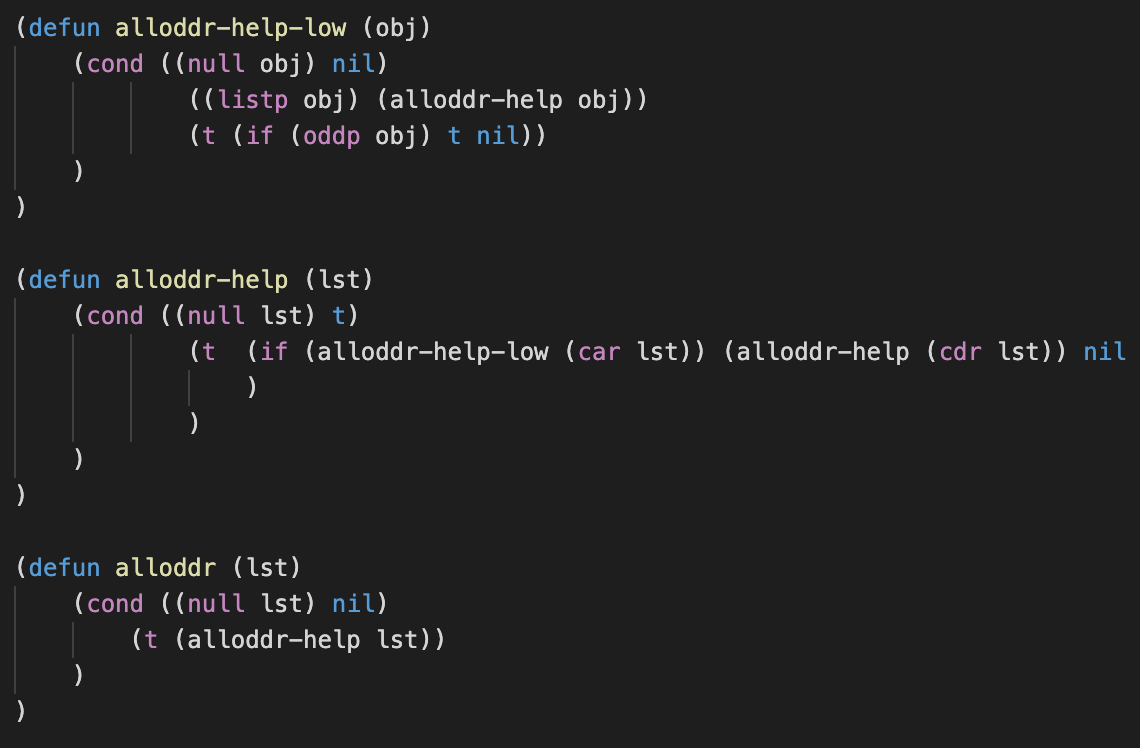
\includegraphics[scale = 0.8]{6.10.png}}
 			\label{ris:6.10}
 		\end{center}
 	\caption{Рекурсивная реализация функции alloddr}
 	\end{figure}
 	
 	\subsection*{Назначение параметров функций}
 	
 	\begin{itemize}
 		\item Функция alloddr - функция-обертка, проверяющая список на nil. Если не пуст, то запускает рекурсиную функцию alloddr-help, где при проверке списка lst на nil, будет возвращаться t, так как будет считаться, что функция перебрала все элементы списка и не нашла ни одного четного
 		\item Функция alloddr-help - рекурсивная функция, проходящая по всем элементам списка и проверяющая с помощью функции alloddr-help-low, является ли какие-нибудь элементы четными или нет
 		\item Функция alloddr-help-low - функция, проверяющая является ли obj списком. Если да, то запускает функцию alloddr-help для него, если нет, то проверяет его на четность нечетность
 	\end{itemize}
 	
 	\subsection*{Результаты работы}
 	
 	 	 	\begin{table} [h!]
 		\begin{center}
 			\begin{tabular}{|l|l|}
 				\hline
 				{\bf  Выражение} & {\bf Результат} \\
 				\hline
 				{'(1 2 3 4 5 6)} & NIL\\
 				\hline
 				{'(1 3 5)} & T\\
 				\hline
 				{'(1)} & T\\
 				\hline
 				{'()} & NIL\\
 				\hline
 				{'(2)} & NIL\\
 				\hline
 				{'(1 3 (5 7))} & T\\
 				\hline
 				{'(1 3 (5 6 7))} & NIL\\
 				\hline
 			\end{tabular}  
 			\label{m2}
 		\end{center}
 	\end{table}
 
 	\newpage
 	
 	\section*{6.11. Написать рекурсивную функцию, относящуюся к хвостовой рекурсии с одним тестом завершения, которая возвращает последний элемент списка - аргументы.
 	}
 	
 	\subsection*{Реализация задания}
 	
 	\begin{figure}[h!]
 		\begin{center}
 			{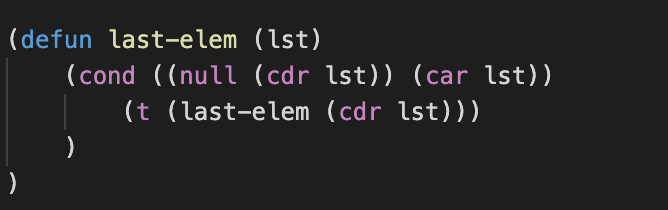
\includegraphics[scale = 1.0]{6.11.png}}
 			\label{ris:6.11}
 		\end{center}
 	\caption{Рекурсивная реализация функции, возвращающей последний элемент списка - аргументы}
 	\end{figure}
 	
 	\subsection*{Назначение параметров функций}
 	
 	\begin{itemize}
 		\item Функция last-elem - рекурсивная функция с одним варинтом завершения - если следующий элемент списка пустой (что означает, что текущий элемент списка - последний)
 	\end{itemize}
 	
 	\subsection*{Результаты работы}
 	
 	 \begin{table} [h!]
 		\begin{center}
 			\begin{tabular}{|l|l|}
 				\hline
 				{\bf  Выражение} & {\bf Результат} \\
 				\hline
 				{'(1 2 3 4 5 6)} & 6\\
 				\hline
 				{'(1 2 3 4 (1 2 3))} & (1 2 3)\\
 				\hline
 				{()} & NIL\\
 				\hline
 			\end{tabular}  
 			\label{m2}
 		\end{center}
 	\end{table}
 	
 	\newpage
 	
 	\section*{6.12. Написать рекурсивную функцию, относящуюся к дополняемой рекурсии с
одним тестом завершения, которая вычисляет сумму всех чисел от 0 до n-ого аргумента функции.
 	}
 
 	Вариант:
 	\begin{enumerate}
 	\item от from-аргумента функции до последнего, 
 	\item от from-аргумента функции до to-аргумента с шагом d.
 \end{enumerate}
 	
 	
 	\subsection*{Реализация задания}
 	
 	Так как в условии задачи не сказано, является ли список-аргумент списком чисел, будем считать, что элементы списка - числа, поскольку реализация функций не сильно изменится (добавится лишь еще одна проверка в cond).
 	
 	 Так как задание лабораторной работы состоит в том, чтобы реализовать поставленные задачи, используя хвостовую рекурсию, было решено использовать ее, а не дополняемую рекурсию, как в условии задачи.
 	
 	\begin{figure}[h!]
 		\begin{center}
 			{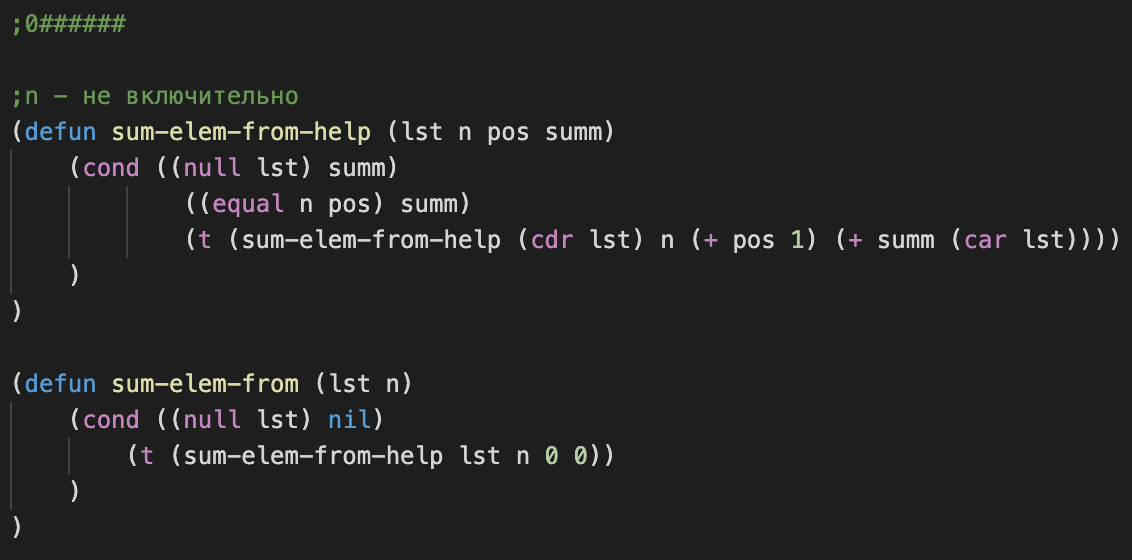
\includegraphics[scale = 0.8]{6.12.0.png}}
 			\label{ris:6.12.0}
 		\end{center}
 	\caption{Рекурсивная реализация функции, вычисляющей сумму всех чисел от 0 до n-ого аргумента функции}
 	\end{figure}
 
  	\begin{figure}[h!]
 	\begin{center}
 		{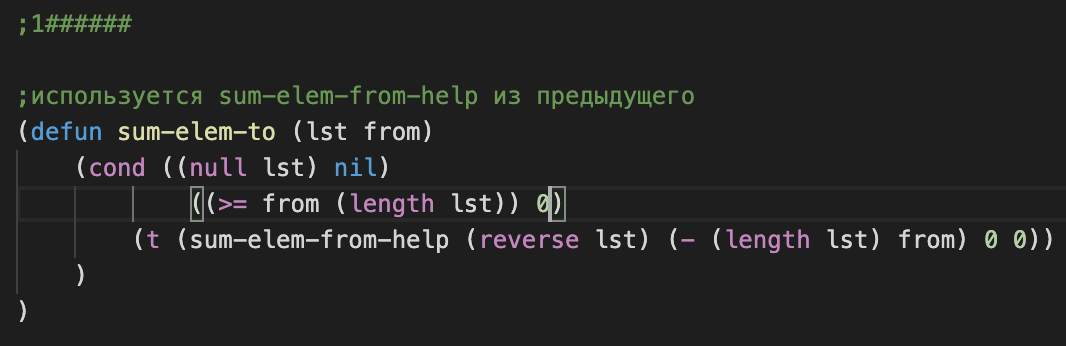
\includegraphics[scale = 0.9]{6.12.1.png}}
 		\label{ris:6.12.1}
 	\end{center}
 \caption{Рекурсивная реализация функции, вычисляющей сумму всех чисел от from-аргумента до последнего}
 \end{figure}

	\newpage
 
  	\begin{figure}[h!]
 	\begin{center}
 		{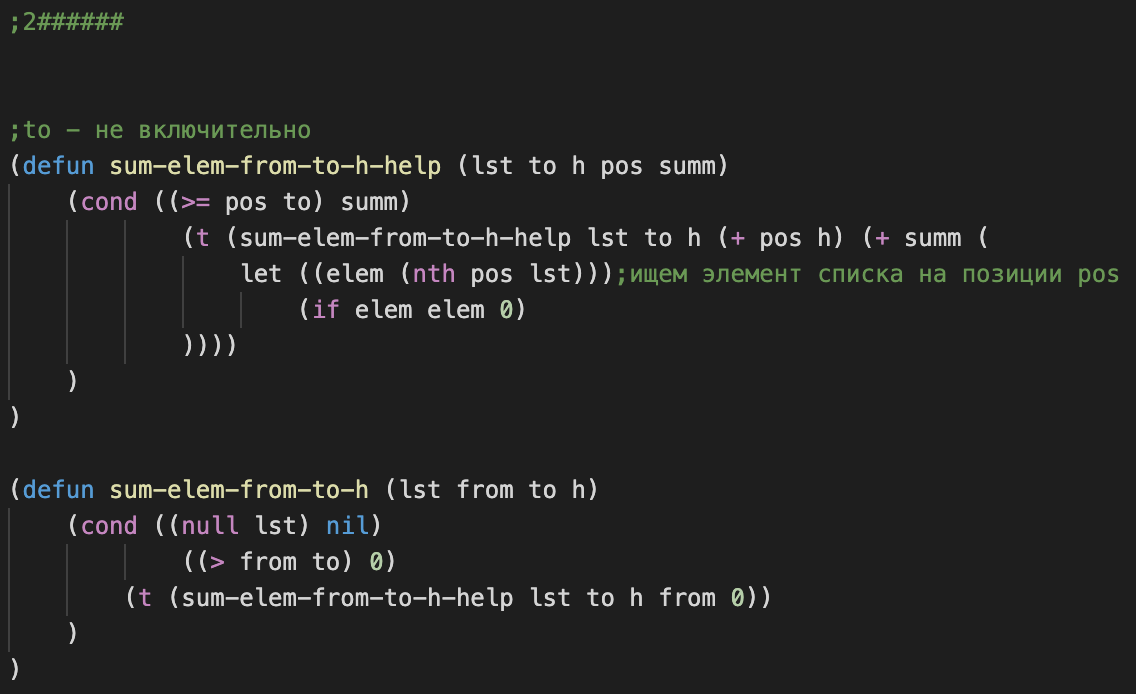
\includegraphics[scale = 0.8]{6.12.2.png}}
 		\label{ris:6.12.2}
 	\end{center}
 \caption{Рекурсивная реализация функции, вычисляющей сумму всех чисел от from-аргумента до to-аргумента с шагом d}
 \end{figure}
 
 	
 	\subsection*{Назначение параметров функций}
 	
 	\begin{itemize}
 		\item Функция sum-elem-from - функция - обертка, проверяющая - пустой ли список lst. Если нет, то запускает рекурсивную функцию sum-elem-from-help с начальными параметрами pos (позиция в списке) = 0, summ (сумма чисел) = 0, иначе nil
 		\item Функция sum-elem-from-help - рекурсивная функция, считающая сумму всех чисел от 0 и до n-ого аргумента функции. Выход из рекурсии осуществляется следующим образом: если список пуст; позиция pos в списке стала равна входному параметру n
 		\item Функция sum-elem-to - функция, аналогичная по логике функции sum-elem-from. Поэтому она переворачивает список lst и вызывает предыдущую функцию sum-elem-from-help с этим списком и (length(lst) - from) позицией в списке, до какой необходимо считать
 		\item Функция sum-elem-from-to-h - функция-обертка, проверяющая - пустой ли список lst, и больше ли параметр from параметра to. Если не пустой, и не больше, то вызывает рекурсивную функцию sum-elem-from-to-h-help с начальными параметрами pos (текущая позиция в списке) = from и summ = 0, иначе nil, если пустой, и 0, если больше
 		\item Функция sum-elem-from-to-h-help - рекурсивная функция, являющаяся по сути реализацией цикла вида: for (int i = from; i < to; i + h) в С++, ищущая на каждой итерации элемент в списке lst на позиции pos с помощью функции nth.
 	\end{itemize}
 	
 	\subsection*{Результаты работы}
 	
    \begin{table} [h!]
 		\begin{center}
 			\begin{tabular}{|l|l|}
 				\hline
 				{\bf  Выражение} & {\bf Результат sum-elem-from} \\
 				\hline
 				{'(1 2 3 4 5 6 7 8) 4} & 10\\
 				\hline
 				{'(1 2 3 4 5 6 7 8) 7} & 36\\
 				\hline
 				{'(1 2 3 4 5 6 7 8) 0} & 0\\
 				\hline
 				{'(1 2 3 4 5 6 7 8) 10} & 36\\
 				\hline
 				{'() 5} & NIL\\
 				\hline
 			\end{tabular}  
 			\label{m2}
 		\end{center}
 	\end{table}
 
 	\begin{table} [h!]
 		\begin{center}
 			\begin{tabular}{|l|l|}
 				\hline
 				{\bf  Выражение} & {\bf Результат sum-elem-to} \\
 				\hline
 				{'(1 2 3 4 5 6 7 8) 4} & 26\\
 				\hline
 				{'(1 2 3 4 5 6 7 8) 7} & 8\\
 				\hline
 				{'(1 2 3 4 5 6 7 8) 0} & 36\\
 				\hline
 				{'(1 2 3 4 5 6 7 8) 10} & 0\\
 				\hline
 				{'() 5} & NIL\\
 				\hline
 			\end{tabular}  
 			\label{m2}
 		\end{center}
 	\end{table}
 
 
 	\begin{table} [h!]
 		\begin{center}
 			\begin{tabular}{|l|l|}
 				\hline
 				{\bf  Выражение} & {\bf Результат sum-elem-from-to-h} \\
 				\hline
 				{'(1 2 3 4 5 6 7 8 9 10) 3 9 1} & 39\\
 				\hline
 				{'(1 2 3 4 5 6 7 8 9 10) 3 9 2} & 18\\
 				\hline
 				{'(1 2 3 4 5 6 7 8 9 10) 3 9 3} & 11\\
 				\hline
 				{'(1 2 3 4 5 6 7 8 9 10) 9 3 1} & 0\\
 				\hline
 				{'(1 3 5 9) 0 4 2} & 6\\
 				\hline
 				{'(1) 0 0 1} & 0\\
 				\hline
 				{'() 0 0 0} & NIL\\
 				\hline
 			\end{tabular}  
 			\label{m2}
 		\end{center}
 	\end{table}
 	
 	\newpage
 	
 	\section*{6.13. Написать рекурсивную функцию, которая возвращает последнее нечетное
число из числового списка, возможно создавая некоторые вспомогательные функции.
 	}
 	
 	\subsection*{Реализация задания}
 	
 	\begin{figure}[h!]
 		\begin{center}
 			{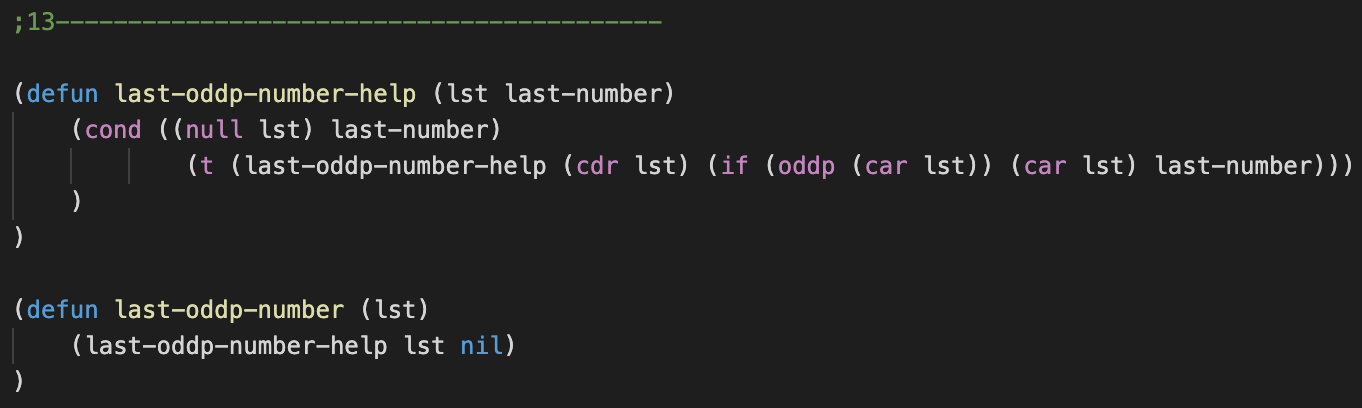
\includegraphics[scale = 0.7]{6.13.png}}
 			\label{ris:6.13}
 		\end{center}
 	\caption{Рекурсивная реализация функции, возвращающей последнее нечетное число из числового списка}
 	\end{figure}
 	
 	\subsection*{Назначение параметров функций}
 	
 	\begin{itemize}
 		\item Функция last-oddp-number - функция - обертка, вызывающая рекурсивную функцию last-oddp-number-help с параметром last-number = nil
 		\item Функция last-oddp-number-help - рекурсивная функция, возвращающая последнее нечетное число из числового списка.
 		\item Если элемент нечетный, то вызываем снова эту функцию с last-number, равным этому элементу
 	\end{itemize}
 	
 	\subsection*{Результаты работы}
 	
 	 	 	\begin{table} [h!]
 		\begin{center}
 			\begin{tabular}{|l|l|}
 				\hline
 				{\bf  Выражение} & {\bf Результат} \\
 				\hline
 				{'(1 2 3 4 5 6 7)} & 7\\
 				\hline
 				{'(1 2 3 4 5 6)} & 5\\
 				\hline
 				{'(1 2 4 6 8 10)} & 1\\
 				\hline
 				{'(2 4 6 8 10)} & NIL\\
 				\hline
 				{'(1)} & 1\\
 				\hline
 				{'(2)} & NIL\\
 				\hline
 				{'()} & NIL\\
 				\hline
 			\end{tabular}  
 			\label{m2}
 		\end{center}
 	\end{table}
 	
 	\newpage
 	
 	\section*{6.14. Используя cons-дополняемую рекурсию с одним тестом завершения,
написать функцию которая получает как аргумент список чисел, а возвращает список квадратов этих чисел в том же порядке.
 	}
 	
 	\subsection*{Реализация задания}
 	
 	Так как задание лабораторной работы состоит в том, чтобы реализовать поставленные задачи, используя хвостовую рекурсию, а в условии задачи, используя cons-дополняемую рекурсию, было решено сделать 2 реализации: используя хвостовую и cons-дополняемую рекурсию.
 	
 	\begin{figure}[h!]
 		\begin{center}
 			{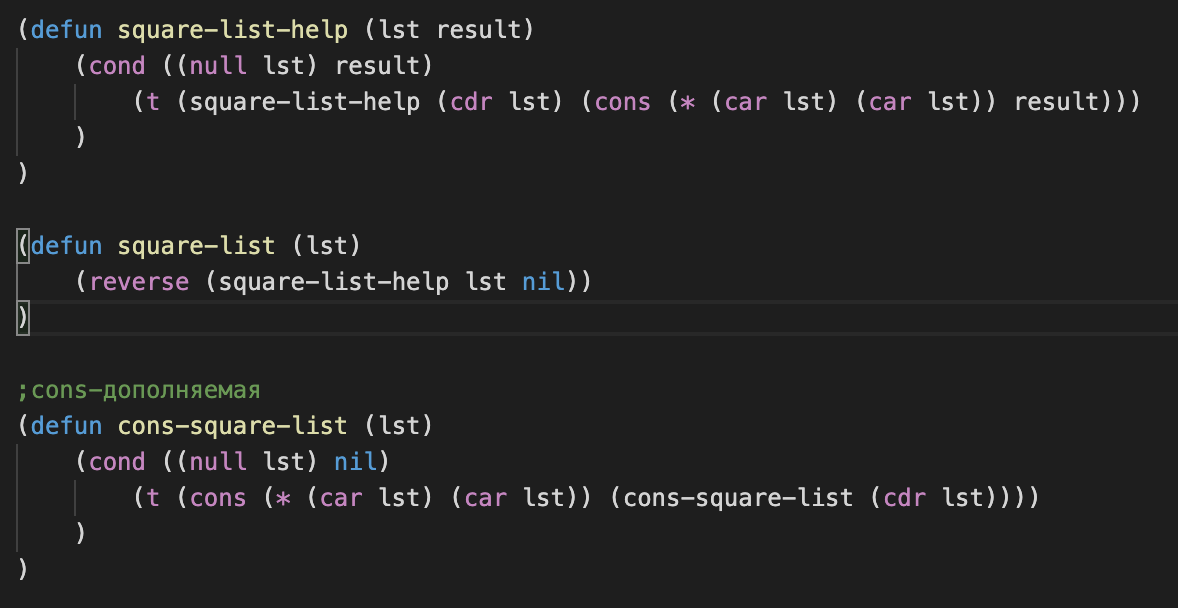
\includegraphics[scale = 0.8]{6.14.png}}
 			\label{ris:6.14}
 		\end{center}
 	\caption{Рекурсивные реализации функций, возвращающих список квадратов чисел-аргументов в том же порядке}
 	\end{figure}
 	
 	\subsection*{Назначение параметров функций}
 	
 	\begin{itemize}
 		\item Функция square-list - функция-обертка, вызывающая рекурсивную функцию square-list-help с начальным параметром result = nil, и переворачивающая результирующий список функцией reverse
 		\item Функция square-list-help - рекурсивная функция, проходящаяся по всем элементам списка, возводя их в квадрат и добавляя их в голову result
 	\end{itemize}
 	
 	\subsection*{Результаты работы}
 	
 	 	 	\begin{table} [h!]
 		\begin{center}
 			\begin{tabular}{|l|l|}
 				\hline
 				{\bf  Выражение} & {\bf Результат} \\
 				\hline
 				{'(1 2 3 4 5 6)} & (1 4 9 16 25 36)\\
 				\hline
 				{'(1 2 3 0)} & (1 4 9 0)\\
 				\hline
 				{'(4)} & (16)\\
 				\hline
 				{'()} & NIL\\
 				\hline
 			\end{tabular}  
 			\label{m2}
 		\end{center}
 	\end{table}
 	
 	\newpage
 	
 	\section*{6.15. Написать функцию с именем select-odd, которая из заданного
списка выбирает все нечетные числа. Вариант 1: select-even, 
вариант 2: вычисляет сумму всех нечетных чисел(sum-all-odd) или сумму всех четных чисел (sum-all-even) из заданного списка.
 	}
 	
 	\subsection*{Реализация задания}
 	
 	Было решено реализовать функции select-odd и sum-all-odd (нечетные числа):
 	
 	\begin{figure}[h!]
 		\begin{center}
 			{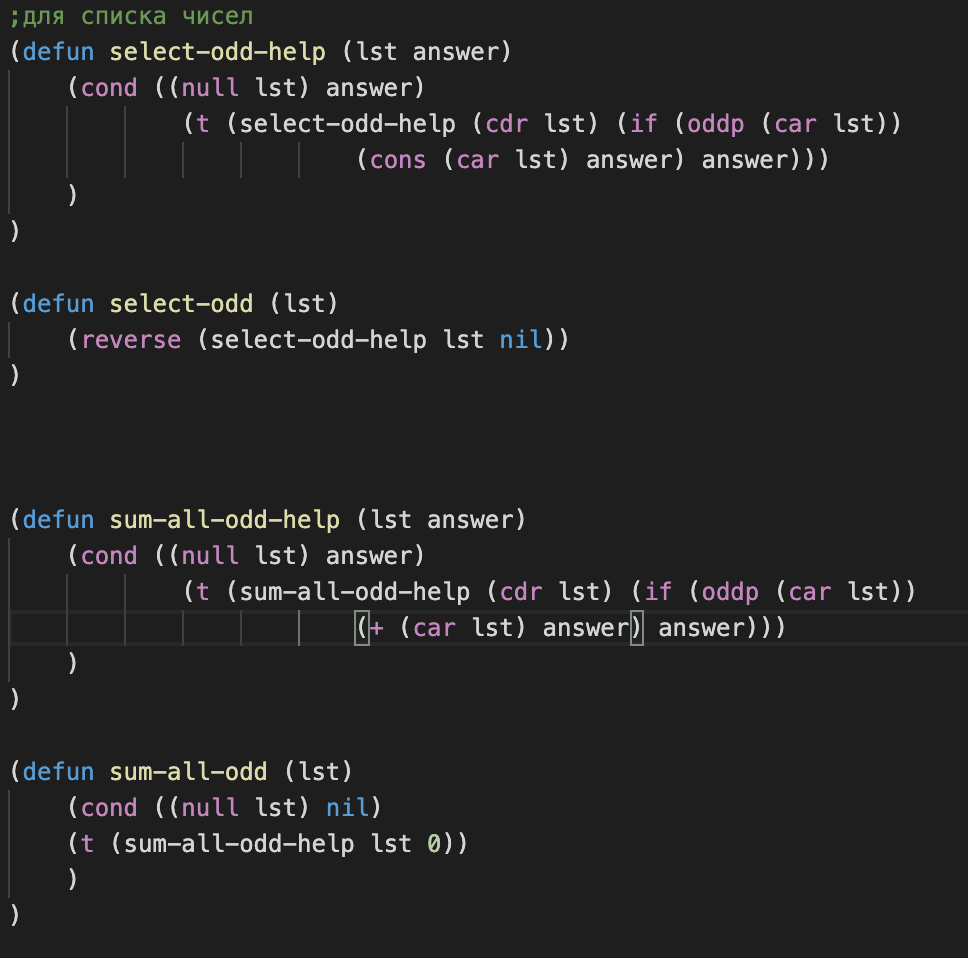
\includegraphics[scale = 0.8]{6.15.1.png}}
 			\label{ris:6.15.1}
 		\end{center}
 	\caption{Рекурсивная реализация функций для списка чисел}
 	\end{figure}
 	
 	\newpage
 	
 	\begin{figure}[h!]
 		\begin{center}
 			{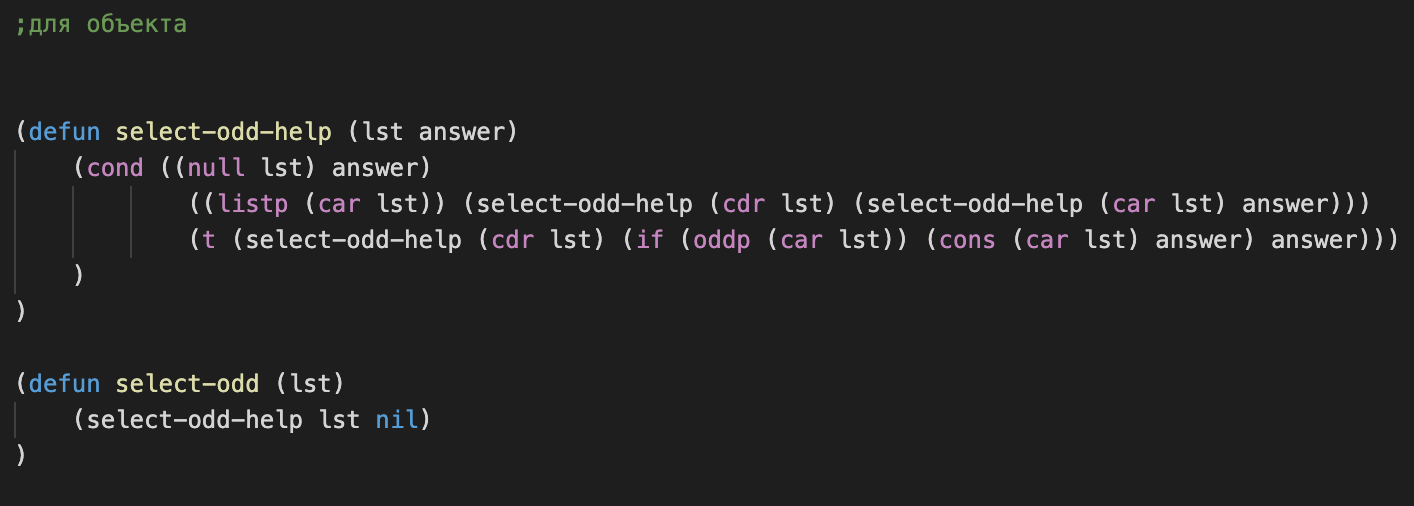
\includegraphics[scale = 0.7]{6.15.2.png}}
 			\label{ris:6.15.2}
 		\end{center}
 	\caption{Рекурсивная реализация функции select-odd для списка объектов}
 	\end{figure}
 	
 	\begin{figure}[h!]
 		\begin{center}
 			{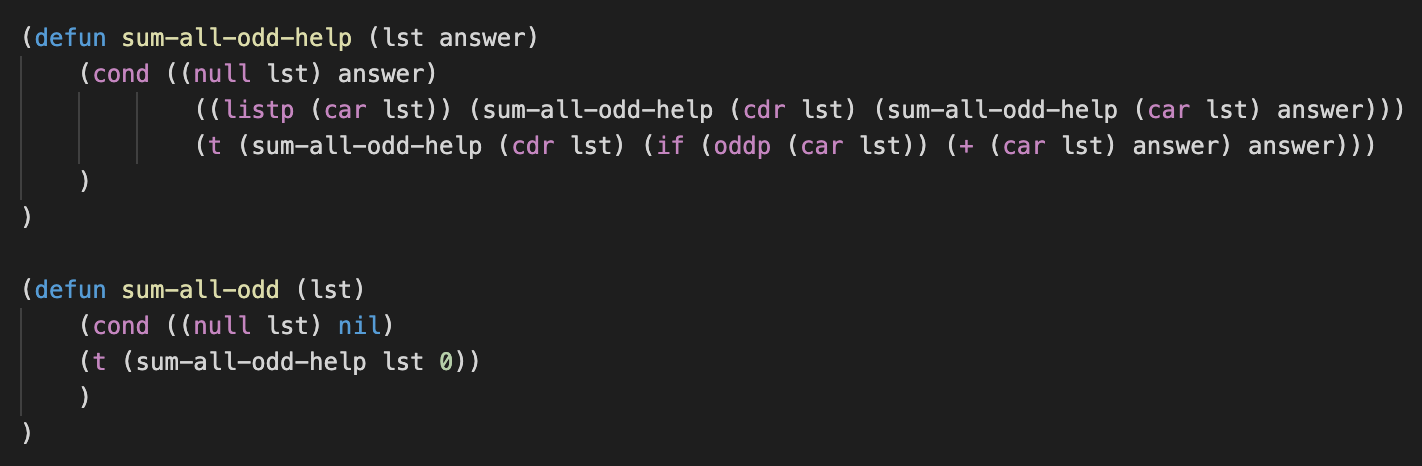
\includegraphics[scale = 0.7]{6.15.3.png}}
 			\label{ris:6.15.3}
 		\end{center}
 	\caption{Рекурсивная реализация функции sum-all-odd для списка объектов}
 	\end{figure}
 	
 	\subsection*{Назначение параметров функций}
 	
 	\begin{itemize}
 		\item Функция select-odd - функция-обертка, вызывающая рекурсивную функцию select-odd-help с начальным параметром answer = nil, и переворачивающая результирующий список функцией reverse
 		\item Функция select-odd-help - рекурсивная функция, проходящаяся по всем элементам списка, проверяющая их на нечетность и добавляя их в голову answer, если нечетное
 		\item Функция sum-all-odd - функция-обертка, проверяющая пустой ли список и вызывающая рекурсивную функцию sum-all-odd-help с начальным параметром answer = 0, если не пуст, иначе nil
 		\item Функция sum-all-odd-help - рекурсивная функция, проходящая по всем элементам списка, проверяющая их на нечетность и прибавляет их к result, если нечетное
 	\end{itemize}
 	
 	\subsection*{Результаты работы}
 	
 	
 	\textit{Функция select-odd:}
 	 \begin{table} [h!]
 		\begin{center}
 			\begin{tabular}{|l|l|l|}
 				\hline
 				{\bf  Выражение} & {\bf Результат для списка чисел} & {\bf Результат для списка объектов} \\
 				\hline
 				{'(1 2 3 4 5 6 7)} & (1 3 5 7) & (1 3 5 7)\\
 				\hline
 				{'(2 4 6)} & NIL & NIL\\
 				\hline
 				{'(1 2 3 4 5 6)} & (1 3 5) & (1 3 5)\\
 				\hline
 				{'(1)} & (1) & (1)\\
 				\hline
 				{'()} & NIL & NIL\\
 				\hline
 				{'(1 2 3 4 5 (3 5) 7)} & --- & (7 5 3 5 3 1)\\
 				\hline
 				{'(1 2 3 4 5 (3 (2) 5) 7)} & --- & (7 5 3 5 3 1)\\
 				\hline
 			\end{tabular}  
 			\label{m2}
 		\end{center}
 	\end{table}
 
 	\textit{Функция sum-all-odd:}
 	\begin{table} [h!]
 		\begin{center}
 			\begin{tabular}{|l|l|l|}
 				\hline
 				{\bf  Выражение} & {\bf Результат для списка чисел} & {\bf Результат для списка объектов} \\
 				\hline
 				{'(1 2 3 4 5 6 7)} & 16 & 16\\
				\hline
				{'(2 4 6)} & 0 & 0\\
				\hline
				{'(1 2 3 4 5 6)} & 9 & 9\\
				\hline
				{'(1)} & 1 & 1\\
				\hline
				{'()} & NIL & NIL\\
				\hline
				{'(1 2 3 4 5 (3 5) 7)} & --- & 24\\
				\hline
				{'(1 2 3 4 5 (3 (2) 5) 7)} & --- & 24\\
				\hline
 			\end{tabular}  
 			\label{m2}
 		\end{center}
 	\end{table}
 	
 	\section*{Ответы на вопросы}
 	
 	\subsection*{Способы организации повторных вычислений в Lisp:}
 	
 	\begin{enumerate}
 		\item Использование функционалов.
 		\item Использование рекурсиии.
 	\end{enumerate}
 	
 	\subsection*{Что такое рекурсия?}
 	
 	\textit{Рекурсия} – это ссылка на определяемый объект во время его определения.
 	
 	\subsection*{Классификация рекурсивных функций в Lisp:}
 	
 	\begin{enumerate}
 		\item Простая рекурсия – один рекурсивный вызов в теле.
 		\item Рекурсия первого порядка – рекурсивный вызов встречается несколько раз.
 		\item Взаимная рекурсия – используется несколько функций, рекурсивно вызывающих друг друга.
 	\end{enumerate}
 	
 	\subsection*{Различные способы организации рекурсивных функций и порядок их реализации.}
 	
 	Способы организации рекурсивных функций:
 	
 	\begin{enumerate}
 		\item \textit{Хвостовая рекурсия.}
 		В целях повышения эффективности рекурсивных функций рекомендуется
 		формировать результат не на выходе из рекурсии, а на входе в рекурсию,
 		все действия выполняя до ухода на следующий шаг рекурсии. Это и есть
 		хвостовая рекурсия.
 		\begin{lstlisting}[label=lst1,caption=Хвостовая рекурсия]
 		( defun fun (x)
 			( cond ( end_test1 end_value1 )
 		 			. . .
 				( end_testN end_valueN )
 				(T ( fun reduced_x ) ) ) )
 		\end{lstlisting}
 		\item \textit{Рекурсия по нескольким параметрам.}
 		\begin{lstlisting}[label=lst2,caption=Рекурсия по нескольким параметрам]
 		( defun fun (n x)
 			( cond ( end_test end_value )
 				(T ( fun ( reduced_n ) ( reduced_x ) ) ) )
 		\end{lstlisting}
 		\item \textit{Дополняемая рекурсия} – при обращении к рекурсивной функции используется дополнительная функция не в аргументе вызова, а вне его.
 		\begin{lstlisting}[label=lst3,caption=Дополняемая рекурсия]
 		( defun fun (x)
 			( cond ( test end_value )
 				(T ( add_fun add_value ( fun reduced_x ) ) ) ) )
 		\end{lstlisting}
 		\item \textit{Множественная рекурсия.} На одной ветке происходит сразу несколько рекурсивных вызовов. Количество условий выхода также может зависеть от задачи.
 		\begin{lstlisting}[label=lst4,caption=Множественная рекурсия]
 		( defun fun (x)
 			( cond ( test end_val )
 				(T ( combine ( fun changed1_x )
 					( fun changed2_x ) ) ) ) )
 		\end{lstlisting}
 	\end{enumerate}
 	
 	\subsection*{Способы повышения эффективности реализации рекурсии.}
 	
 	В целях повышения эффективности рекурсивных функций рекомендуется
 	формировать результат не на выходе из рекурсии, а на входе в рекурсию, все
 	действия выполняя до ухода на следующий шаг рекурсии. Это и есть хвостовая
 	\textit{рекурсия}.
 	
 	Для превращения не хвостовой рекурсии в хвостовую и в целях формирования результата (результирующего списка) на входе в рекурсию рекомендуется
 	использовать дополнительные (рабочие) параметры. При этом становится необходимым создать функцию-оболочку для реализации очевидного обращения к
 	функции.
 	
 	

\end{document}